
\section{Analiza sistema}

	U sklopu poslovanja ne spada samo dostava namirnica do klijenta već i nabavka namirnica od snabdevača i njihovo skladištenje po magacinima. U nastavku opisujemo aktere koje prepoznajemo i koje su njihove uloge u sistemu.

\subsection{Akteri}
	\begin{itemize}
		\item{\textbf{Klijent}} - predstavlja krajnjeg korisnika. Klijent nakon registracije postavlja inicijalna podešavanja profila: tip obroka, broj porcija i broj obroka po nedelji. Na osnovu ovih podataka formira se cena pretplate i ova podešavanja se pamte. Klijent ima mogućnost menjanja ovih podataka u budućnosti i svaki put se cena formira na osnovu njih. U okviru podešavanja inicijalnih podataka, unosi podatke o dostavi i načinu plaćanja, nakon čega bira obroke. Na osnovu izabranih obroka formira se spisak potrebnih namirnica i njihova količina koje će mu biti dostavljene. Takođe, ovi podaci mogu biti naknadno izmenjeni. Klijent može u bilo kom trenutku otkazati pretplatu i preskočiti dostavu za narednu nedelju. U sklopu paketa dostavljaju se i recepti za obrok, napisani korak po korak. Klijentu se svake nedelje menja ponuda mogućih obroka. Sistem je zaslužan za pravljenje ponude i to radi po određenom algoritmu koji bira obroke i njihove recepte iz baze podataka. Klijent može odabrati datum i vreme dostave, međutim vreme dostave je podložno promeni u periodu do sat vremena od unete satnice, zbog dostupnosti dostavljača.
		\item{\textbf{Dostavljač}} - preuzima pakete sa liste isporuka za taj dan. U slučaju kašnjenja dostave, obaveštava klijenta.
		\item{\textbf{Magacioner}} - pakuje pakete koji treba da se dostave u toku nedelje. Prima dostavljene namirnice i raspoređuje ih po magacinu.
		\item{\textbf{Koordinator}} - zadužen je za kontrolu magacina, koliko i kojih namirnica dolazi i odlazi iz magacina. U slučaju nedostatka određenih namirnica mora da kontaktira snabdevače kako bi ih nabavio.
		\item{\textbf{Snabdevač}} - proizvodi određene namirnice i u obavezi je da dostavi koordinatoru određenu količinu namirnica na njegov zahtev. Ima pristup sistemu, ali ne predstavlja zapošljeno lice u kompaniji ChooseFresh.
		\item{\textbf{Administrator}} - objavljuje konkurs za snabdevače, pravi ugovor o saradnji sa snabdevačima i zapošljava nova lica. 
		
		U daljem tekstu pod terminom \textit{zapošljena lica} podrazumevamo dostavljača, magacionera i koordinatora, dok pod terminom \textit{korisnici} podrazumevamo sve aktere u sistemu. Na slici \ref{fig:context_diagram} prikazan je dijagram konteksta na kome su predstavljeni svi akteri sistema.
		
				
	\end{itemize}
\subsection{Dijagram toka podataka}

\begin{figure}[H]
	\begin{center}
		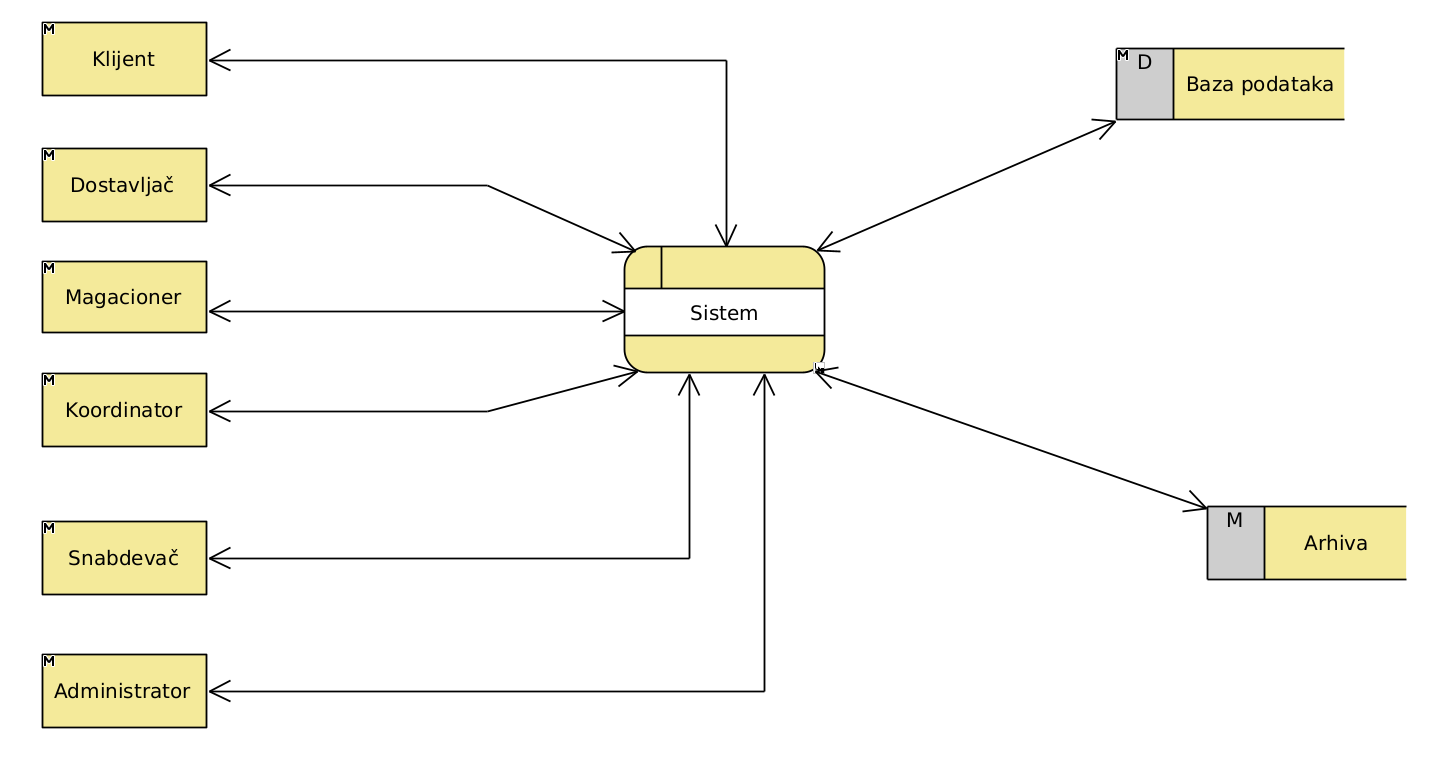
\includegraphics[width=\textwidth]{context_diagram.png}

	    \caption{Dijagram konteksta}
	\label{fig:context_diagram}
    \end{center}
    
\end{figure}

	Na slici \ref{fig:DFD} prikazan je dijagram toka podataka nivoa 0. U nastavku su ukratko objašnjeni procesi predstavljeni dijagramom.
	
	
	\textbf{Upravljanje nalozima}: Ovim procesom je obuhvaćena registracija klijenta i zaposlenih, kao i prijavljivanje korisnika sistemu. Uključuje ažuriranje i brisanje naloga klijenta, zaposlenih i snabdevača.
	
	\textbf{Odabir i ažuriranje plana ishrane}: Podrazumeva inicijalni odabir plana ishrane klijenta koji se pretplaćuje, kao i proces kasnijeg ažuriranja plana ishrane.
		
	\textbf{Dostava paketa}: Uključuje proces zakazivanja isporuka, pakovanja paketa i dostave paketa klijentu. 
	
	
	\textbf{Nabavka namirnica}: Koordinator naručuje namirnice od snabdevača koji ih doprema do magacina, zatim magacioner raspoređuje primljene namirnice i vodi evidenciju o primljenim namirnicama.
	
	
	\textbf{Prijava i registracija snabdevača}: Ovaj proces je drugačiji od registracije klijenta i zaposlenih jer zahteva dodatne podatke (izveštaj inspekcije, prijavu snabdevača dobijenu apliciranjem snabdevača, i dokumentaciju snabdevača).


\begin{figure}[H]
	\begin{center}
		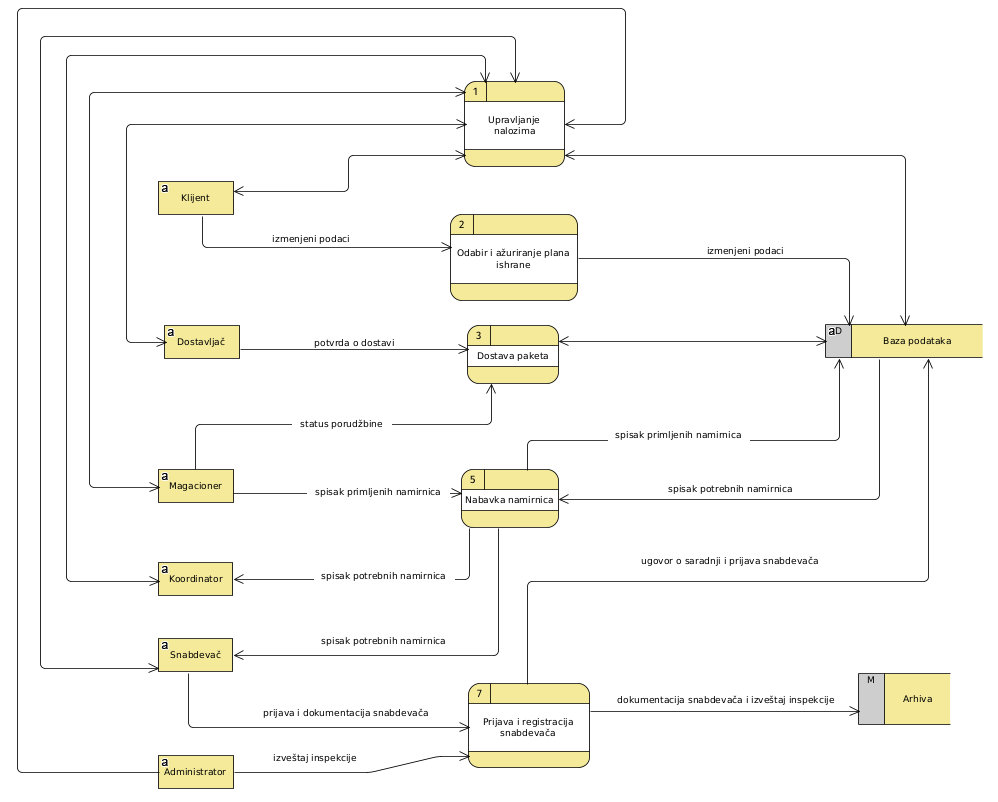
\includegraphics[width=\textwidth]{dfd.png}

    		\caption{Dijagram toka podataka nivoa 0}
    \label{fig:DFD}
    \end{center}
 
\end{figure}

	
